
%(BEGIN_QUESTION)
% Copyright 2006, Tony R. Kuphaldt, released under the Creative Commons Attribution License (v 1.0)
% This means you may do almost anything with this work of mine, so long as you give me proper credit

Determine the following voltage drops in this level-sensing circuit when the process level is at a height of 12 feet.  Note that this is {\it not} a loop-powered transmitter, but receives its electrical power through separate power conductors (120 volts AC).  Assume negligible (0) voltage drop along the signal conductor lengths:

$$\includegraphics[width=15.5cm]{i00293x01.eps}$$

\begin{itemize}
\item{} Voltage drop across transmitter signal terminals = 
\item{} Voltage drop between TB40-3 and TB27-21 = 
\item{} Voltage drop across 250 $\Omega$ resistor = 
\item{} Voltage drop between TB12-3 and TB27-21 = 
\end{itemize}

\vskip 20pt \vbox{\hrule \hbox{\strut \vrule{} {\bf Suggestions for Socratic discussion} \vrule} \hrule}

\begin{itemize}
\item{} Demonstrate how to {\it estimate} numerical answers for this problem without using a calculator.
\item{} If the voltage drop along the signal wiring length were significant rather than zero, how would the voltage calculations be affected?  Would significant loop wire resistance cause a level measurement error?  If so, would it result in a {\it high} error or a {\it low} error?
\item{} Explain why this particular level transmitter must be self-powered rather than loop-powered as is (more) typical for process transmitters.
\item{} Explain why non-contact radar level transmitters must be used only on metal vessels in order to comply with FCC regulations, while guided-wave radar level transmitters may be used in either metal or non-metal vessels.
\item{} As process level increases, will the voltage measured across the transmitter's terminals {\it increase}, {\it decrease}, or {\it remain the same}?
\item{} Suppose this self-powered (``4-wire'') level transmitter were replaced be a loop-powered (``2-wire'') level transmitter.  As process level increases, will the voltage measured across the transmitter's terminals {\it increase}, {\it decrease}, or {\it remain the same}?
\end{itemize}

\underbar{file i00293}
%(END_QUESTION)





%(BEGIN_ANSWER)

\noindent
{\bf Partial answer:}

\begin{itemize}
\item{} Voltage drop across transmitter signal terminals =
\item{} Voltage drop between TB40-3 and TB27-21 = 
\item{} Voltage drop across 250 $\Omega$ resistor = {\bf 2.6 volts}
\item{} Voltage drop between TB12-3 and TB27-21 = 
\end{itemize}

%(END_ANSWER)





%(BEGIN_NOTES)

A liquid height of 12 feet in a 0-30 foot range yields the following percentage:

$${12 \hbox{ ft} \over 30 \hbox{ ft}} = 40\%$$

This 40\% translates into a 10.4 milliamp DC signal sent to the indicator, producing a 2.6 volt DC drop across the 250 $\Omega$ resistor.

\begin{itemize}
\item{} Voltage drop across transmitter terminals = {\bf 2.6 volts}
\item{} Voltage drop between TB40-3 and TB27-21 = {\bf 2.6 volts} 
\item{} Voltage drop across 250 $\Omega$ resistor = {\bf 2.6 volts}
\item{} Voltage drop between TB12-3 and TB27-21 = {\bf 0 volts} 
\end{itemize}

\vskip 20pt \vbox{\hrule \hbox{\strut \vrule{} {\bf Virtual Troubleshooting} \vrule} \hrule}

This question is a good candidate for a ``Virtual Troubleshooting'' exercise.  Presenting the diagram to students, you first imagine in your own mind a particular fault in the system.  Then, you present one or more symptoms of that fault (something noticeable by an operator or other user of the system).  Students then propose various diagnostic tests to perform on this system to identify the nature and location of the fault, as though they were technicians trying to troubleshoot the problem.  Your job is to tell them what the result(s) would be for each of the proposed diagnostic tests, documenting those results where all the students can see.

During and after the exercise, it is good to ask students follow-up questions such as:

\begin{itemize}
\item{} What does the result of the last diagnostic test tell you about the fault?
\item{} Suppose the results of the last diagnostic test were different.  What then would that result tell you about the fault?
\item{} Is the last diagnostic test the best one we could do?
\item{} What would be the ideal order of tests, to diagnose the problem in as few steps as possible?
\end{itemize}

%INDEX% Basics, line-powered transmitter: voltage drop calculations

%(END_NOTES)


